% Experiment section: learning-augmented densest at-most-k subgraph.
% Requires: booktabs, graphicx, subcaption. Figures in figures/.
% References to Lemma 3.1, Algorithm 3 and Theorem 3.4 are written as plain
% numbers; replace with \ref{...} to match the paper's labels.

\section{Densest At-Most-$k$ Subgraph on Twitch Ego-Nets}
\label{sec:exp-damks}

\paragraph{Setup.} We evaluate the learning-augmented densest at-most-$k$ subgraph
algorithm (Algorithm 3), which we denote \textsc{LA-DamkS}, on 500 ego-nets from the Twitch Ego Nets
collection~\cite{karateclub2020}, with $30 \le n \le 52$ (mean $n = 40.4$, mean $m = 136.9$)
and $k = 15$. Edges are treated as undirected. The ground truth $H^\star$ is computed exactly by
Dinkelbach's method~\cite{dinkelbach1967}: given the current best set with $e$ edges on $s$
vertices, we solve the integer program
\[
\max\; s\textstyle\sum_{uv\in E} y_{uv} - e\sum_{v\in V} x_v
\quad\text{s.t.}\quad y_{uv}\le x_u,\ y_{uv}\le x_v,\ 1\le\textstyle\sum_v x_v\le k,\ x\in\{0,1\}^V,
\]
strengthened with the valid inequalities
$\sum_{u\in N(v)} y_{uv}\le \min\{\sum_w x_w - x_v,\ (k-1)x_v\}$, using HiGHS~\cite{highs}.
All coefficients are integers, so a positive optimum yields a strictly denser set, and an optimum
of $0$ certifies that the current set is optimal. All 500 instances are solved to proven
optimality, with $5 \le |H^\star| \le 15$.

\paragraph{Models and evaluation.} A random forest (100 trees) predicts
$p(v) \sim \mathbf{1}[v\in H^\star]$ from five per-vertex features: degree, average
neighbor degree, number of vertices, core number, and local clustering coefficient.
Following Lemma 3.1, the predicted set is $S = \{v : p(v)\ge 1/2\}$. \textsc{LA-DamkS} needs
$\varepsilon$, which we estimate as the mean of $|S\,\triangle\,H^\star|/|H^\star|$ on a held-out
$20\%$ calibration split of the training graphs; this gives
$\hat\varepsilon\in[0.44, 0.48]$ across folds. We use 5-fold cross-validation over
graphs, so every graph is evaluated by a model that has not seen it. The main baseline,
\emph{predictor only}, returns $S$ itself. We also report top-$k$, the $k$ vertices with the
largest $p(v)$, which is always feasible.

\paragraph{Results.} Table~\ref{tab:damks-quality} reports the ratio $d(\cdot)/d(H^\star)$.
The predictor is weak: its mean normalized error is $|S\,\triangle\,H^\star|/|H^\star| = 0.48$,
far outside the small-$\varepsilon$ regime of Theorem 3.4. Moreover, $S$ is infeasible
($|S| > k$) on 205 of the 500 graphs. Even so, \textsc{LA-DamkS} reaches a mean ratio of $0.937$
(median $0.996$) and is exactly optimal on $48.4\%$ of the graphs. Predictor only reaches
$0.817$ even when its infeasible outputs are scored at face value. Restricted to graphs where
$S$ is feasible, it reaches only $0.705$. Per graph, \textsc{LA-DamkS} beats predictor only on 387
graphs, ties on 7 and loses on 106; in 86 of those losses, $S$ was infeasible.

The expansion step is what drives the gain. With $\varepsilon$ fixed rather than estimated,
the mean ratio increases monotonically from $0.813$ at $\varepsilon=0$ (only trimming $S$ to
$k$) to $0.891$, $0.923$, $0.938$ and $0.950$ at $\varepsilon = 0.1, 0.3, 0.5, 0.6$
(Figure~\ref{fig:damks}b). Overestimating $\varepsilon$ is therefore inexpensive here: adding
more vertices with many edges into $S$ costs little, because trimming removes the weakly
attached ones.

\begin{table}[t]
\centering
\begin{tabular}{lccccc}
\toprule
method & mean & median & min & $\ge 0.95$ & optimal \\
\midrule
\textsc{LA-DamkS} ($\hat\varepsilon$)         & \textbf{0.937} & \textbf{0.996} & 0.250 & \textbf{74.6\%} & \textbf{48.4\%} \\
predictor only, at face value          & 0.817 & 0.907 & 0.000 & 35.0\% & 18.2\% \\
predictor only, $|S|\le k$ ($n{=}295$) & 0.705 & 0.810 & 0.000 & 14.2\% & 2.7\% \\
top-$k$ by $p(v)$                      & 0.894 & 0.913 & 0.532 & 27.4\% & 6.6\% \\
\bottomrule
\end{tabular}
\caption{Ratio $d(\cdot)/d(H^\star)$ on 500 Twitch ego-nets ($k = 15$, 5-fold
cross-validation). ``At face value'' also counts the 205 graphs where $|S| > k$, so it
overstates that baseline.}
\label{tab:damks-quality}
\end{table}

\begin{table}[t]
\centering
\begin{tabular}{lrrrrr}
\toprule
 & mean & median & 90th pct & max & total \\
\midrule
exact ILP                    & 213 ms   & 17.9 ms  & 617 ms   & 4480 ms & 107 s \\
\textsc{LA-DamkS} (end-to-end)     & 0.289 ms & 0.290 ms & 0.414 ms & 1.06 ms & 0.144 s \\
\bottomrule
\end{tabular}
\caption{Time per graph over the 500 graphs, single-threaded. The time for \textsc{LA-DamkS}
includes feature computation and forest inference but excludes the one-time training of the
forest; the algorithm alone takes 0.009 ms on average.}
\label{tab:damks-time}
\end{table}

\begin{figure}[t]
\centering
\begin{subfigure}{0.49\textwidth}
  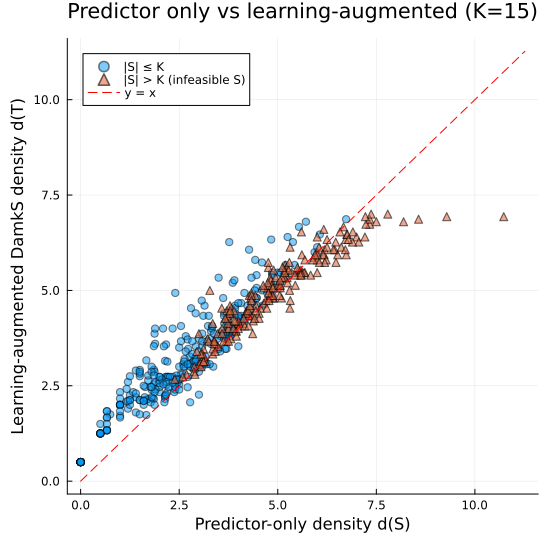
\includegraphics[width=\linewidth]{figures/damks_pred_predictor_vs_algorithm.png}
  \caption{}
\end{subfigure}\hfill
\begin{subfigure}{0.49\textwidth}
  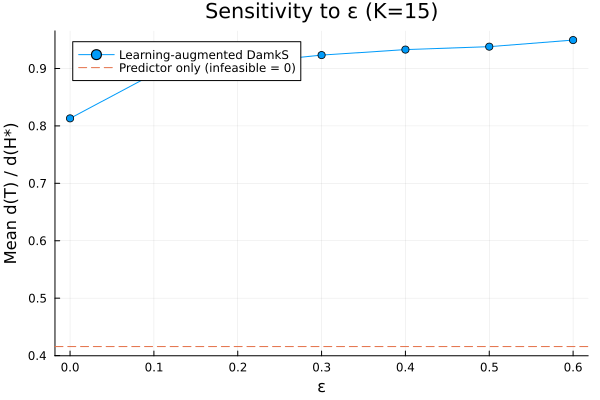
\includegraphics[width=\linewidth]{figures/damks_pred_eps_sweep.png}
  \caption{}
\end{subfigure}
\caption{(a) Per-graph density of predictor only vs.\ \textsc{LA-DamkS}. Triangles mark graphs with
infeasible $S$. (b) Mean ratio of \textsc{LA-DamkS} for a fixed $\varepsilon$.}
\label{fig:damks}
\end{figure}

\paragraph{Running time.} Table~\ref{tab:damks-time} compares \textsc{LA-DamkS} with computing
$H^\star$ exactly by the integer program. Both run single-threaded on the same machine.
\textsc{LA-DamkS} is $74\times$ faster per graph (median), at least $19.5\times$ faster on every
graph, and $738\times$ faster in total. The integer program's cost grows quickly with graph
size and has a heavy tail: its mean time rises from 82\,ms for $n\in[30,39]$ to 417\,ms for
$n\in[47,52]$. Over the same range, \textsc{LA-DamkS} stays between 0.24 and 0.34\,ms with no loss in
quality (mean ratio $0.940$ and $0.948$ respectively).
